\documentclass[handout]{beamer}

\usepackage{ts-glærur}

\title{FOR3R - Endurkvæmni}

\begin{document}
\begin{frame}
\titlepage
\end{frame}

\section{Inngangur}

\begin{frame}{Hvað er endurkvæmni?}
\pause
\begin{itemize}
 \item Endurkvæmt reiknirit (e. \emph{recursive algortithm}) er hvert það reiknirit sem kallar á sjálft sig \pause
 \item Af hverju viljum við það? \pause
 \begin{itemize}
  \item Hugmynd: Vegna þess að stundum getur það gefið okkur góða lýsingu á vandamálum og eðli þeirra.
 \end{itemize}
\end{itemize}
\end{frame}

\begin{frame}{Divide and Conquer}
Introduction to Algorithms lýsir divide-and-conquer - almenn lausnaraðferð sem notar endurkvæmni.
\begin{itemize}
 \item  \textbf{Divide} the problem into a number of subproblems that are smaller instances of the
same problem.
 \item \textbf{Conquer} the subproblems by solving them recursively. If the subproblem sizes are
small enough, however, just solve the subproblems in a straightforward manner.
 \item \textbf{Combine} the solutions to the subproblems into the solution for the original problem.
\end{itemize}
Getum við séð fyrir okkur leið til að nota þessa aðferð?
\end{frame}


\begin{frame}[fragile]{Dæmi: Factorial}
``Hrópmerkt''-fallið er auðvelt að skilgreina á endurkvæman máta:

\begin{minted}{python}
def r_factorial(n):
    if n <= 1:
        return 1
    else:
        return n*r_factorial(n-1)
\end{minted}
Hér er grunntilfellið $n=1$. Kallað er á ``smærra'' tilvik af vandamálinu í síðustu línunni. 
\end{frame}

\section{Jafngildi }

\begin{frame}[fragile]{Factorial með lykkju?}
Er líka hægt að leysa þetta með lykkju?
\pause
Já, það er álíka auðvelt.
\begin{minted}{python}
def i_factorial(n):
    result = 1
    for i in range(1, n+1):
        result *= i
    return result
\end{minted}
Sama reiknirit, önnur útfærsla.

\pause
Spurning: Er þetta \emph{alltaf} hægt?
\end{frame}

\begin{frame}{Jafngildi}
\begin{itemize}
 \item Staðhæfing: Endurkvæmni og ítrun geta leyst sama mengi vandamála
 \begin{itemize}
  \item Ekki sannað hér, en hugmyndir:
  \begin{itemize}
   \item Ítrun yfir í endurkvæmni: Breyta breytum í lykkju í fallsviðföng
   \item Endurkvæmni yfir í ítrun: Halda utan um stöðuna með því að búa til eigin ``hlaða''
  \end{itemize}
 \end{itemize}
 \item Þetta þýðir að alltaf er hægt að breyta endurkvæmu reikniriti í reikniriti sem notar ítrun og öfugt
 \item Á einnig við GOTO
 \item Allt saman eru þetta mismunandi leiðir til að lýsa sömu reikningum
\end{itemize}
\pause
Spurning: Hvað eigum við að nota?
\end{frame}

\begin{frame}{Viðeigandi notkun}
\begin{itemize}
 \item Uppástunga: Í praxís, notið það sem ykkur finnst auðveldast að útfæra
 \item Leyfið forritunarmálinu að sjá um bestun
 \begin{itemize}
  \item Þið gætuð endað með sama vélamálskóðann hvort sem er
  \item Bestið ef hraði eða minnisnotkun er ófullnægjandi skv. \emph{mælingum}
 \end{itemize}
 \item Íhugið endurkvæmni ef hægt er að skipta undirvandamálinu upp í smærri vandamál sem eru sama eðlis
 \begin{itemize}
  \item Dæmi: Helmingunarleit
 \end{itemize}
\end{itemize}
\end{frame}

\section{Fleiri hugtök í endurkvæmni}

\subsection{Hlaðinn}

\begin{frame}{``Hlaðinn''}
\begin{columns}
\column{0.55\textwidth}
\begin{itemize}
 \item Í mörgum (flestum?) forritunarmálum er haldið utan um fallsköll á hlaða (e. \emph{stack})
 \begin{itemize}
  \item Safn af upplýsingum um hvert fallskall á að snúa þegar því er lokið
 \end{itemize}
 \item Áberandi í endurkvæmni: Til að búa til nýja færslu á hlaðanum þarf tíma og minni
\end{itemize}
\column{0.45\textwidth}
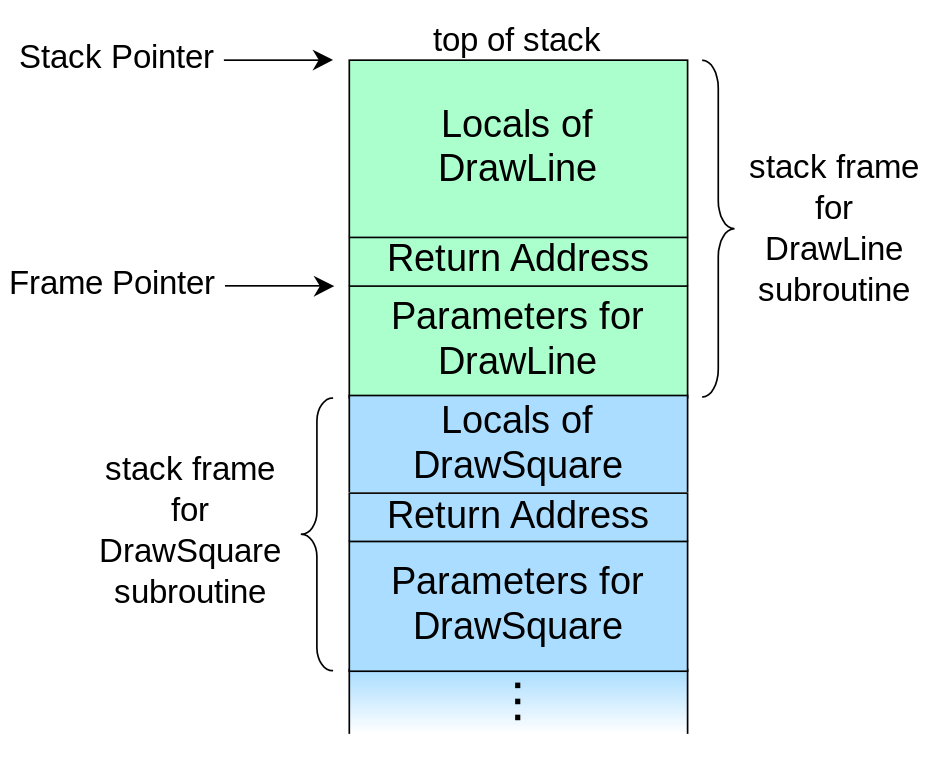
\includegraphics[width=\linewidth]{Pics/call-stack}
\end{columns}

\end{frame}


\subsection{Halaendurkvæmni}
\begin{frame}{Halaendurkvæmni}
\begin{columns}
\column{0.6\textwidth}
\begin{itemize}
 \item Mikilvægt hugtak í endurkvæmni er halaendurkvæmni (e. \emph{tail recursion})
 \item Um halaendurkvæmni er að ræða þegar endurkvæmt fall \emph{endar} á kalli á sjálft sig
 \begin{itemize}
  \item Fallið á þá ekki inni frekari útreikninga
 \end{itemize}
 \item Í halaendurkvæmri útfærslu er hægt að henda vísuninni í ``foreldri''  fallskalssins
 \begin{itemize}
  \item Hægt að útfæra á hagkvæmari máta!
  \item Gert í sumum forritunarmálum
 \end{itemize}
\end{itemize}
\pause 

\column{0.4\textwidth}
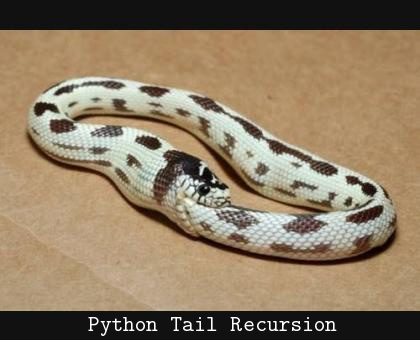
\includegraphics[width=\linewidth]{Pics/pythontailrecursion}
\end{columns}
\end{frame}

\begin{frame}[fragile]{Halaendurkvæmni: Dæmi}
\begin{minted}{python}
def tail_factorial(n,total = 1):
    if n <= 1:
        return total
    else:
        return tail_factorial(n-1,total*n)
\end{minted}
Ath: Fallið er aldrei að bíða eftir öðrum fallsköllum
\end{frame}


\begin{frame}{Stuðningur við hagkvæma halaendurkvæmni}
Niðurstöður örstuttrar gúglrannsóknar:
\begin{itemize}
 \item Python: \href{http://neopythonic.blogspot.com/2009/04/tail-recursion-elimination.html}{Nei}
 \item C\#: Nei (F\#: Já)
 \item C++: Já (með optimization flags)
 \item Java: Nei (Scala: Já)
 \item JavaScript: Nei
 \item PHP: Nei
 \item Lisp/Scheme: Já
\end{itemize}
\end{frame}

\subsection{Hjálparföll}
\begin{frame}{Hjálparföll}
\begin{itemize}
 \item Hjálparföll eru oft notuð inni í ``fallegri'' föllum til að fela endurkvæmnina
 \item Einnig má líta á það sem svo að endurkvæma fallið sé aðalfallið, fallið sem notandinn sér bara hjúpur
 \item Þetta er sérstaklega algengt í halaendurkvæmum föllum, sem oft þurfa að halda utan um ``stöðuupplýsingar'' í inntökunum
\end{itemize}
\end{frame}

\begin{frame}[fragile]{Hjálparföll - dæmi}
\begin{minted}{python}
def tail_list_reverse(my_list, rev_list):
    n = len(my_list)
    if n == 0:
        return rev_list
    else:
        rev_list.insert(0, my_list.pop(0))
        return tail_list_reverse(my_list, rev_list)


def pretty_list_reverse(my_list):
    return tail_list_reverse(my_list,[])
\end{minted}
\end{frame}


\subsection{Multiple recursion, single recursion}

\begin{frame}{Multiple, single}

\begin{itemize}
 \item Talað er um multiple recursion og single recursion
 \begin{itemize}
  \item Single recursion: Fallið kallar á sjálft sig einu sinni
  \item Multiple recursion: Fallið kallar oftar en einu sinni á sjálft sig
 \end{itemize}
 \item Dæmi um multiple recursion: Beint-af-augum endurkvæm útfærsla á Fibonacci reikniritinu
\end{itemize}
\end{frame}

\section{Tenglar}
\begin{frame}{Tenglar}
SO þræðir:
\begin{itemize}
 \item \href{http://stackoverflow.com/q/2093618/1675015}{Can all iterative algorithms be expressed recursively?}
 \item \href{http://stackoverflow.com/q/159590/1675015}{Way to go from recursion to iteration}
 \item \href{http://stackoverflow.com/q/2651112/1675015}{Is recursion ever faster than looping?}
 \item \href{http://stackoverflow.com/q/33923/1675015}{What is tail recursion?}
 \item \href{http://stackoverflow.com/q/310974/1675015}{What is tail call optimization?}
\end{itemize}

\end{frame}

\end{document}
